\documentclass[a4j,11pt]{jarticle}
%\usepackage[dviout]{graphicx}
\usepackage[dvipdfmx]{graphicx}
\usepackage{amsmath}
\usepackage{amssymb}
\usepackage{ascmac}
%\usepackage{epsbox}
\usepackage{float}
\usepackage{here}
\usepackage{lscape}
\usepackage{latexsym}
\usepackage{pifont}
\usepackage{wrapfig}
\usepackage{type1cm}
\usepackage{algorithm}
\usepackage{algorithmic}
\usepackage{txfonts}
\usepackage{bm}
\usepackage{comment}
\usepackage{url}
%\usepackage{natbib}
%\usepackage[square]{natbib}

\usepackage{listings}
%\usepackage{plistings}

%\setlength{\voffset}{-25.4mm}
\setlength{\topmargin}{-17.5mm}   %トップとヘッダの間隔
%\setlength{\headheight}{20mm}   %ヘッダの高さ
%\setlength{\headsep}{0mm}   %ヘッダとテキストの間隔
\setlength{\textwidth}{45zw}   %テキストの幅
\setlength{\hoffset}{-10mm}
\setlength{\textheight}{45\baselineskip}   %テキストの高さ
%\addtolength{\textheight}{\topskip}
%\setlength{\footskip}{0mm}
%\setlength{\oddsidemargin}{21.5mm}   %サイドとテキストの間隔(奇数ページ)
%\setlength{\evensidemargin}{21.5mm}   %サイドとテキストの間隔(偶数ページ)
\pagestyle{empty}   %ページ番号なし
\newcommand{\g}[1]{\boldsymbol{#1}}
\newcommand{\lw}[1]{\smash{\lower2.0ex\hbox{#1}}}
\renewcommand{\baselinestretch}{1.0}

\makeatletter
\def\theequation{\arabic{equation}}   %数式番号を(章.式)形式
\@addtoreset{equation}{section}
%\def\thefigure{\thesection.\arabic{figure}}   %図番号を(章.図)形式
%\@addtoreset{figure}{section}
%\def\thetable{\thesection.\arabic{table}}   %表番号を(章.表)形式
%\@addtoreset{table}{section}
\def\tr{\mathop{\operator@font tr}\nolimits}
\def\grad{\mathop{\operator@font grad}\nolimits}
\def\St{\mathop{\operator@font St}\nolimits}
\def\Hess{\mathop{\operator@font Hess}\nolimits}
\def\D{\mathop{\operator@font D}\nolimits}
\def\sym{\mathop{\operator@font sym}\nolimits}
\def\s.t.{\mathop{\operator@font s.t.}\nolimits}
\def\diag{\mathop{\operator@font diag}\nolimits}
\def\section{\@startsection{section}{1}{\z@}
   {0.8\Cvs \@plus.5\Cdp \@minus.2\Cdp}
   {0.2\Cvs \@plus.3\Cdp}
   {\normalfont \Large \bfseries}}
\makeatother
\makeatletter
\def\subsection{\@startsection{subsection}{1}{\z@}
   {0.8\Cvs \@plus.5\Cdp \@minus.2\Cdp}
   {0.2\Cvs \@plus.3\Cdp}
   {\normalfont \normalsize \bfseries}}
\makeatother
\makeatletter
\newcommand{\figcaption}[1]{\def\@captype{figure}\caption{#1}}
\newcommand{\tblcaption}[1]{\def\@captype{table}\caption{#1}}
\makeatother

\begin{document}
%\bibliographystyle{jecon} %参考文献に番号ふらない
%\bibliographystyle{apalike} %いらない

\begin{center}
{\Large \textbf{混合射影正規分布によるクラスタリングについて}}
\end{center}
\begin{flushright}
小坪 琢人(塩濱 敬之准教授)
\end{flushright}
\vspace{-3zh}

%%%%%%%%%%%%% これ以下, 本文 %%%%%%%%%%%5%%
%%%%%%%%%%%%%  section1  はじめに %%%%%%%%%%%%%%%

\section{はじめに}



\section{超球面上のクラスタリング}

$k$平均法は, 各データと各クラスタの中心のユークリッド距離を最小化することで, 各データをクラスタリングする. しかし確率変数が円周上や球面上に値をとるようなデータに対して, ユークリッド空間のクラスタリングを前提とした$K$平均法はしばしば誤った分類結果をもたらす. Dhillon and Modha(2001) は, ユークリッド距離に基づく非類似度の尺度を単位球面上に射影したコサイン非類似度の最小化に基づく超球面上の$k$平均法を提案した. このようなベクトルを角度データと呼ぶ. データの単位方向ベクトルと各クラスタにおける重心ベクトルとのコサイン非類似度を最小化することで, 各データをクラスタリングする. 

超球面上の$k$平均法は確率モデルを仮定しないノンパラメトリックな手法であるのに対し,  パラメトリックな超球面上のクラスタリング手法として, Gopal and Yang(2014) による von Mises Fisher 分布の混合分布を用いた手法がある. 混合ガウスモデルと同様に, データが von Mises Fisher 分布の混合分布から発生した際に, 混合モデルのパラメータをマルコフ連鎖モンテカルロ法(MCMC)によりサンプリングする. MCMCを用いることで求める事後分布のパラメータの平均値, 標準偏差を求めることができる. 本研究では方向データの分布として知られる, 射影正規分布の混合分布によるクラスタリングの性能評価を行う. %以下要確認%
射影正規分布はパラメータによって, 単峰性・二峰性の形状を取ることができるので, 多峰性のデータをクラスタリングする際に混合 von Mises Fisher 分布によるクラスタリングとどのような差異が現れるか比較する.

%%%%%%%%%%%%%%%%%%%%%%%%%%%%%%%%%%%%%%%%%%%%%%%%%%%%%%%%%%%%%%%%%%%%%%%%%%%%%%%%%%%%%%%%%%%%%%%%%%%%%%%%%%%%%%%
%%%%%%%%%%%%%%%%%%%%%%%% senction2 混合分布 %%%%%%%%%%%%%%%%%%%%%

\section{混合 Projected Normal 分布}
\vspace{-0.5zh}
\subsection{Projected Normal 分布}

射影分布は平面または空間上の放射状の射影によって得られる. 一般的には, 多変量正規ベクトルをノルムで割ることで, 単位超球面上への射影分布が得られる. 多変量正規ベクトル($k$次元)を$X$として, $k \geq 2$ の場合には, 単位超球面上への単位ベクトル $U$ は $U = X/||X||$ で表される. このとき$U$は$k$次元の一般化射影正規分布に従い, $U \sim \mathcal{PN}_k(\bm \mu,\Sigma)$と表せる. 一般化射影正規分布は, パラメータ$\bm \mu, \Sigma$をもち, Presnell(1998) らによる, $\Sigma = \mathcal{I}$と定義されていた, 射影正規分布を一般化したものである. $\mathcal{PN}_k(\bm \mu,\mathcal{I})$は平均方向$\bm \mu$に対して, 単峰性かつ対称の分布となるが, $\mathcal{PN}_k(\bm \mu,\Sigma)$では対称分布もしくは二峰性分布となる.

Wang and Gelfand (2013) によると, $\Sigma \neq I$のもとで$\mathcal{PN}_2(\bm \mu,\Sigma$)のとき, 円形データの場合, 単位円上の方向を表す$U = (\cos\Theta, \sin\Theta)^T$における$\theta$の確率密度は以下で表す.

\vspace{-1zh}
\begin{eqnarray*}
\label{PNC}
p(\theta; \bm \mu, \Sigma) = \frac{1}{2\pi A(\theta)}|\Sigma|^{-\frac{1}{2}}
\exp(C)\left\{1 + \frac{B(\theta)}{\sqrt{A(\theta)}} \frac{\Phi \left(\frac{B(\theta)}{\sqrt{A(\theta)}}\right)}{\phi \left(\frac{B(\theta)}{\sqrt{A(\theta)}}\right)}\right\} I_{[0,2\pi)}(\theta)
\end{eqnarray*}

\noindent
ここで, $\bm u^T = (\cos\theta,\sin\theta), A(\theta) = \bm u^T\Sigma^{-1}\bm u, B(\theta) = \bm u^T \Sigma^{-1} \bm \mu, C = -\frac{1}{2} \bm \mu^T \Sigma^{-1} \bm \mu$であり, $I_{[0,2\pi)} (\cdot)$は指示関数, $\Phi(\cdot),\phi(\cdot)$ は標準正規分布の確率密度関数と累積密度関数である. 

\newpage
\vspace{-0.5zh}
\subsection{混合 Projected Normal 分布}

$m$個のユニットからなる 射影正規分布の混合分布は以下のように定式化できる. 

\vspace{-2zh}
\begin{eqnarray*}
p(\theta;\bm w,\bm \mu, \Sigma) = \sum^m_{j=1} w_j \mathcal{PN}_2(\theta;\bm \mu_j, \Sigma_j) 
\end{eqnarray*}

\vspace{-1zh}
\noindent
ただし, $w_j$は混合比率であり, $0 < w_j < 1$, $\sum^m_{j=1} w_j = 1$を満たす. ここで両辺の対数を取ると, 

\vspace{-2zh}
\begin{eqnarray}
\label{logPN}
\log p(\theta;\bm w,\bm \mu, \Sigma)  &=& \sum^m_{j=1} \{\log w_j + \log \mathcal{PN}_2(\theta;\bm \mu_j, \Sigma_j)\} \nonumber \\ 
&=& \sum^m_{j=1} \left[ \log w_j - \log 2\pi - \log A - \frac{1}{2} \log |\Sigma| + C + \log \left\{1 + \frac{B(\theta)}{\sqrt{A(\theta)}} \frac{\Phi \left(\frac{B(\theta)}{\sqrt{A(\theta)}}\right)}{\phi \left(\frac{B(\theta)}{\sqrt{A(\theta)}}\right)}\right\} \right] \nonumber \\
&\propto& \sum^m_{j=1} \left[ \log w_j - \log A - \frac{1}{2} \log |\Sigma| + C + \log \left\{1 + \frac{B(\theta)}{\sqrt{A(\theta)}} \frac{\Phi \left(\frac{B(\theta)}{\sqrt{A(\theta)}}\right)}{\phi \left(\frac{B(\theta)}{\sqrt{A(\theta)}}\right)}\right\} \right]  
\end{eqnarray}

\vspace{-0.5zh}\noindent
最後の式変形では, 対数尤度を計算するときに, 定数項は尤度に影響を与えないので消去する.

%%%%%%%%%%%%%%%%%%%%%%%%%%%%%%%%%%%%%%%%%%%%%%%%%%%%%%%%%%%%%%%%%%%
%%%%%%%%%%%%%%%%%%%%%%%  sectio3 解析手法 %%%%%%%%%%%%%%%%%%%%%%%%

\section{解析手法}

\vspace{-0.5zh}
\subsection{マルコフ連鎖モンテカルロ法}

本研究ではMCMCアルゴリズムの一つである, ハミルトニアン$\cdot$モンテカルロ法(HMC)を用いて分布の推定を行う. HMCのアルゴリズムはハミルトン方程式の数学的性質によって正当性が保証されている. 一般の確率分布からのサンプリングについて, ハミルトン方程式を定義するには, 元の問題に存在しない仮想的な運動量を補助変数として導入する必要がある. 

HMCは物理学の考えを用いて, メトロポリスアルゴリズムによるランダムウォークな振る舞いを局所的に抑圧する. 従って, 目標の分布までより素早く推移することを可能にする. 対象となる各確率変数 $(\theta_j)$に対して, 速度変数$\phi_j$を付与する. このメトロポリスアルゴリズムでは$\theta, \phi$を共に更新する. $\theta$の分布の推移には$ \phi$が大きく影響する. 

HMCでは, 事後確率$p(\theta|y)$は$p(\phi)$の独立な分布によって増大する. したがって結合分布を以下のように定義する.

\vspace{-1zh}
\begin{eqnarray*}
p(\theta, \phi|y) = p(\phi)p(\theta|y)
\end{eqnarray*}

$\theta$をシュミレーションするために, 上記の結合分布によりパラメータをシュミレーションする. この補助変数$\phi$を導入することでパラメータ空間をより効率的に移動することを可能にする. HMCは対数事後密度の勾配を要求する. $d$次元のパラメータ$\theta$の勾配は以下で表す.

\vspace{-1zh}
\begin{eqnarray*}
\frac{d \log p(\bm \theta|y)}{d \bm \theta} = \left( 
  \frac{d \log p(\bm \theta|y)}{d \theta_1}, \ldots,
  \frac{d \log p(\bm \theta|y)}{d \theta_d} \right)
\end{eqnarray*}

$\phi$については, 平均$0$, 共分散行列$M$の多変量正規分布を与える. $\phi$の要素が独立の場合は各次元ごとに$\phi_j \sim N(0,M_{jj})$を与える. $M$は,事後分布の逆共分散行列 $\Bigl(\mbox{var}(\theta|y)\Bigr)^{-1}$で大まかにスケールすることができる. しかし, アルゴリズムはどんな場合でも動作するが, $M$のスケーリングが優れているだけで, HMCがより効率的となる.

HMCでは3つの動作を繰り返し行う.

\begin{enumerate}

\item{}
この反復は, $\phi$をその事後分布から無作為に引くことによって開始する. これは, $\phi \sim N(0,M)$の事前分布と同様である.

\item{}
$\theta, \phi$を同時に更新する.
\vspace{-0.5zh}
\begin{eqnarray*}
\phi_{t+\frac{1}{2}} \leftarrow \phi_t + \frac{1}{2} \epsilon \frac{d \log p(\theta|y)}{d\theta}, 
\theta{t+1} \leftarrow \theta_t + \epsilon M^{-1}\phi_{t+\frac{1}{2}},
\phi_{t+1} \leftarrow \phi_{t+\frac{1}{2}} + \frac{1}{2} \epsilon \frac{d \log p(\theta|y)}{d\theta_{t+1}}. 
\end{eqnarray*}

\item{}
得られたパラメータの採択, 棄却を決定する. 上記のステップで得られたパラメータを$\theta^*, \phi^*$として,
現在が$t$回目の反復とすると, サンプルの棄却率は
\vspace{-0.5zh}
$$ r = \frac{p(\theta^*|y) p(\phi^*)}{p(\theta^{t-1}|y) p(\phi^{t-1})}$$
と定義され, $0$から$1$の間でランダムに選んだ数値より, $r$が高ければ$\theta^*$を採択する. サンプル数が定めた値に達したら, 終了する.

\end{enumerate}

\vspace{-0.5zh}
\subsection{パラメータの推定手法}

Projected Normal 分布におけるパラメータは, $\bm \mu,\Sigma$ であるが, 識別可能性を保持するという制約を加えると, 共分散行列$\Sigma$は以下で定義される.
\vspace{-0.5zh}
\[
 \Sigma = \left(
    \begin{array}{cc}
      \tau^2 & \rho \tau \\
      \rho \tau & 1
    \end{array}
  \right)
\]

よって推定すべきパラメータは$\bm \mu, \tau, \rho, \bm w$となる. Wang and Gelfand (2013)の研究から, 各パラメータの事前分布を $\bm \mu \sim N(\bm 0, 10^5 \bm I_2)$, $\tau \sim \mathrm{half Cauchy}(0,5)$, $\rho \sim U(-1,1)$, $\bm w \sim Dirichlet(2,2, \cdots, 2)$ と設定する. ここで重みパラメータ$\bm w$は$m$次元の$Dirichlet$分布に従うものとする. MCMCのアルゴリズムに従って, 各パラメータを変化させながら, 式$\ref{logPN}$で定義した対数尤度を最大化するようなパラメータの分布を取得する. パラメータは収束すると, 単峰性の分布となり, その平均値をパラメータの推定値として扱うことが出来る. 

%%%%%%%%%%%%%%%%%%%%%%%%%%%%%%%%%%%%%%%%%%%%%%%%%%%%%%%%%%%%%%%%%%%
%%%%%%%%%%%%%%%%%%%%%%%  sectio4 数値実験 %%%%%%%%%%%%%%%%%%%%%%%%

\section{シミュレーション}

人工的データを用いて, 混合 Projected Normal 分布によるクラスタリングの性能評価を行う. 複数の von Mises 分布に従う乱数を発生させて, 1つのデータにまとめることで混合データを作成する. 

\subsection{解析データ}

$\mu(0 < \mu < 2\pi), \kappa(\kappa \geq 0) $をパラメータ, $\theta(0 \leq \theta < 2\pi)$を確率変数とする, Von Mises 分布の確率密度関数は以下の式で表せる. また式中の第一種変形ベッセル関数の定義式を示す.

\vspace{-1zh}
\begin{eqnarray*}
f(\theta;\mu, \kappa) = \frac{\exp[\kappa \cos(\theta - \mu)]}{2 \pi I_0(\kappa)} , I_j(\kappa) = \left(\frac{\kappa}{2}\right)^j \sum^\infty_{i=0} \frac{\left(\frac{\kappa^2}{4}\right)^i}{i \Gamma(j + i + 1)}
\end{eqnarray*}

ユニット数$m=4$, 角度$\theta = \left( \frac{7\pi}{4}, \frac{2\pi}{3}, \frac{5\pi}{4}, \frac{\pi}{6}\right)$, パラメータ$\kappa= (2,10,5,15)$, 混合比率$(0.4, 0.2, 0.3, 0.1)$として, 乱数を生成する. 

\vspace{-1zh}
\begin{figure}[H]
\begin{center}
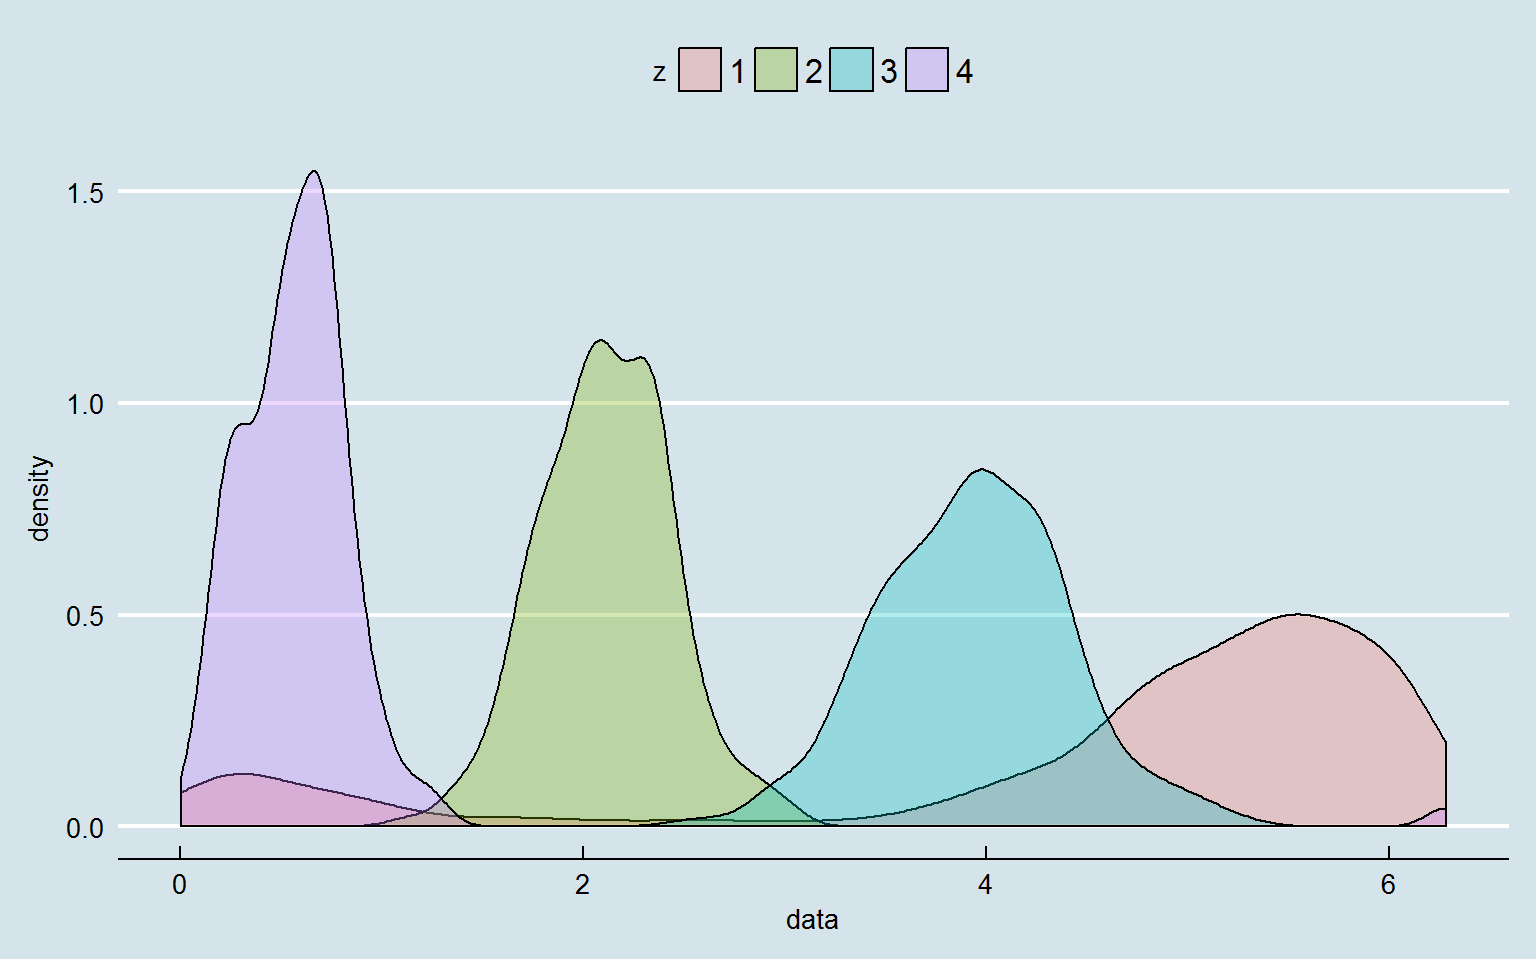
\includegraphics[clip,height= 35mm]{data/mix_test_data.png}
\end{center}
\caption{混合データ(クラスター数:4)}

\label{mixdata}
\end{figure}

\subsection{解析結果}

Mixture von Mises 分布では元のデータと同じく4つの元となる分布を推定したが, Mixture Projected Normal 分布においては3つの元となる分布により以下の結果が得られた.

\begin{figure}[h]
 \begin{tabular}{c}
\hspace{0.5cm}
 \begin{minipage}{0.5\hsize}
  \begin{center}
   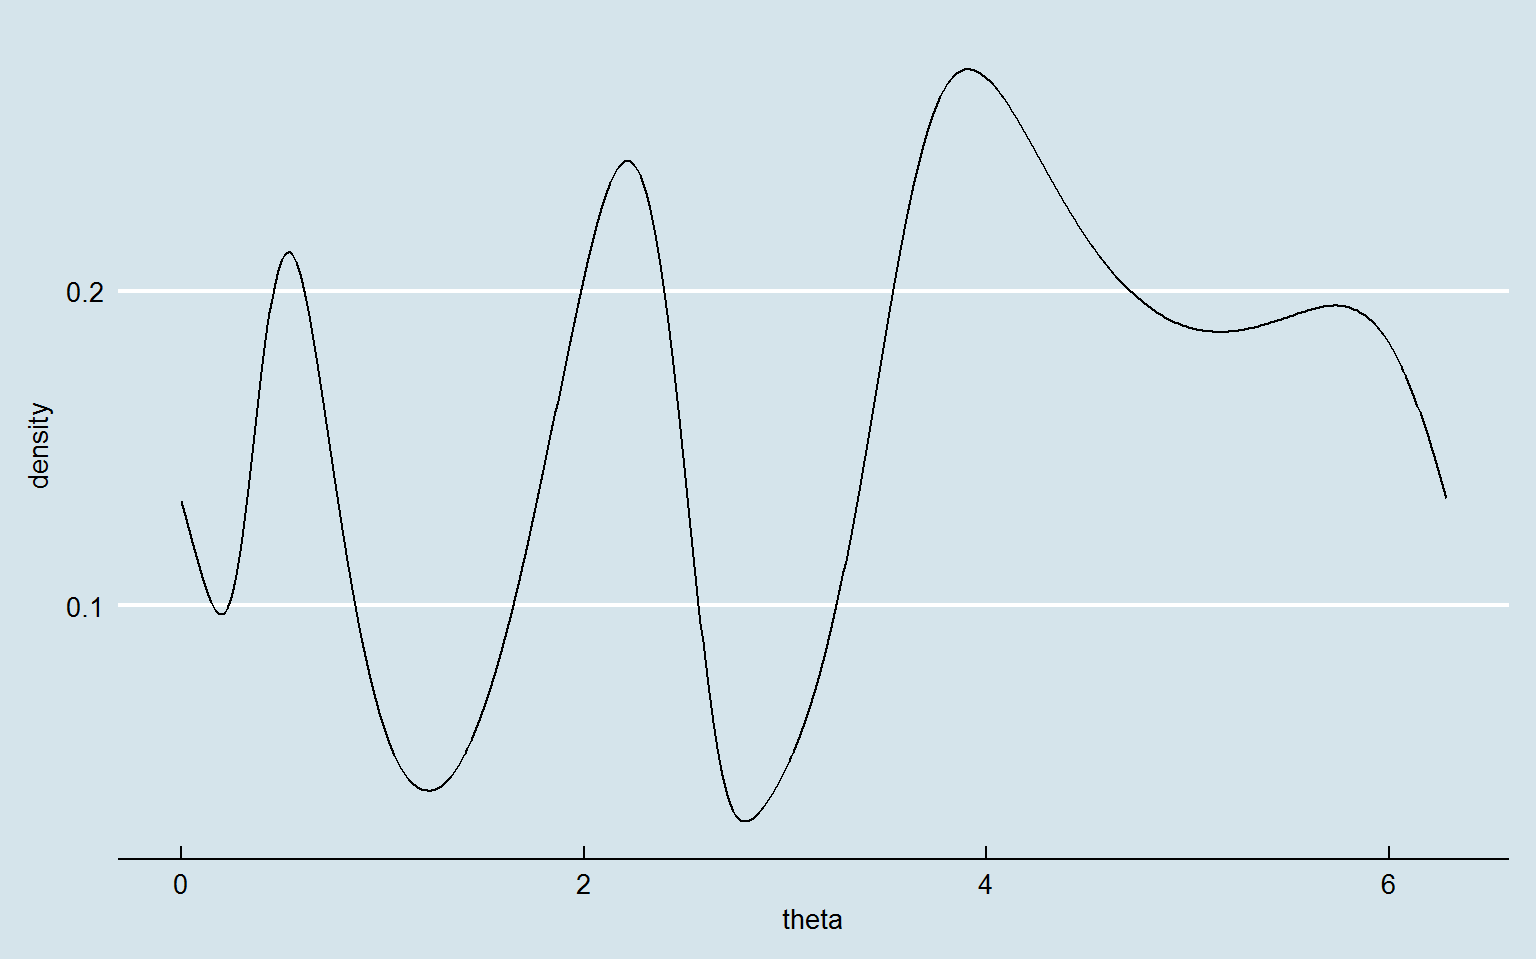
\includegraphics[clip,height= 35mm]{data/mix_pn.png}
  \end{center}
  %\caption{Mixture Projected Normal 分布により推定した混合分布}
  \label{pnmix}
 \end{minipage}
\hspace{-1.0cm}
 \begin{minipage}{0.5\hsize}
  \begin{center}
   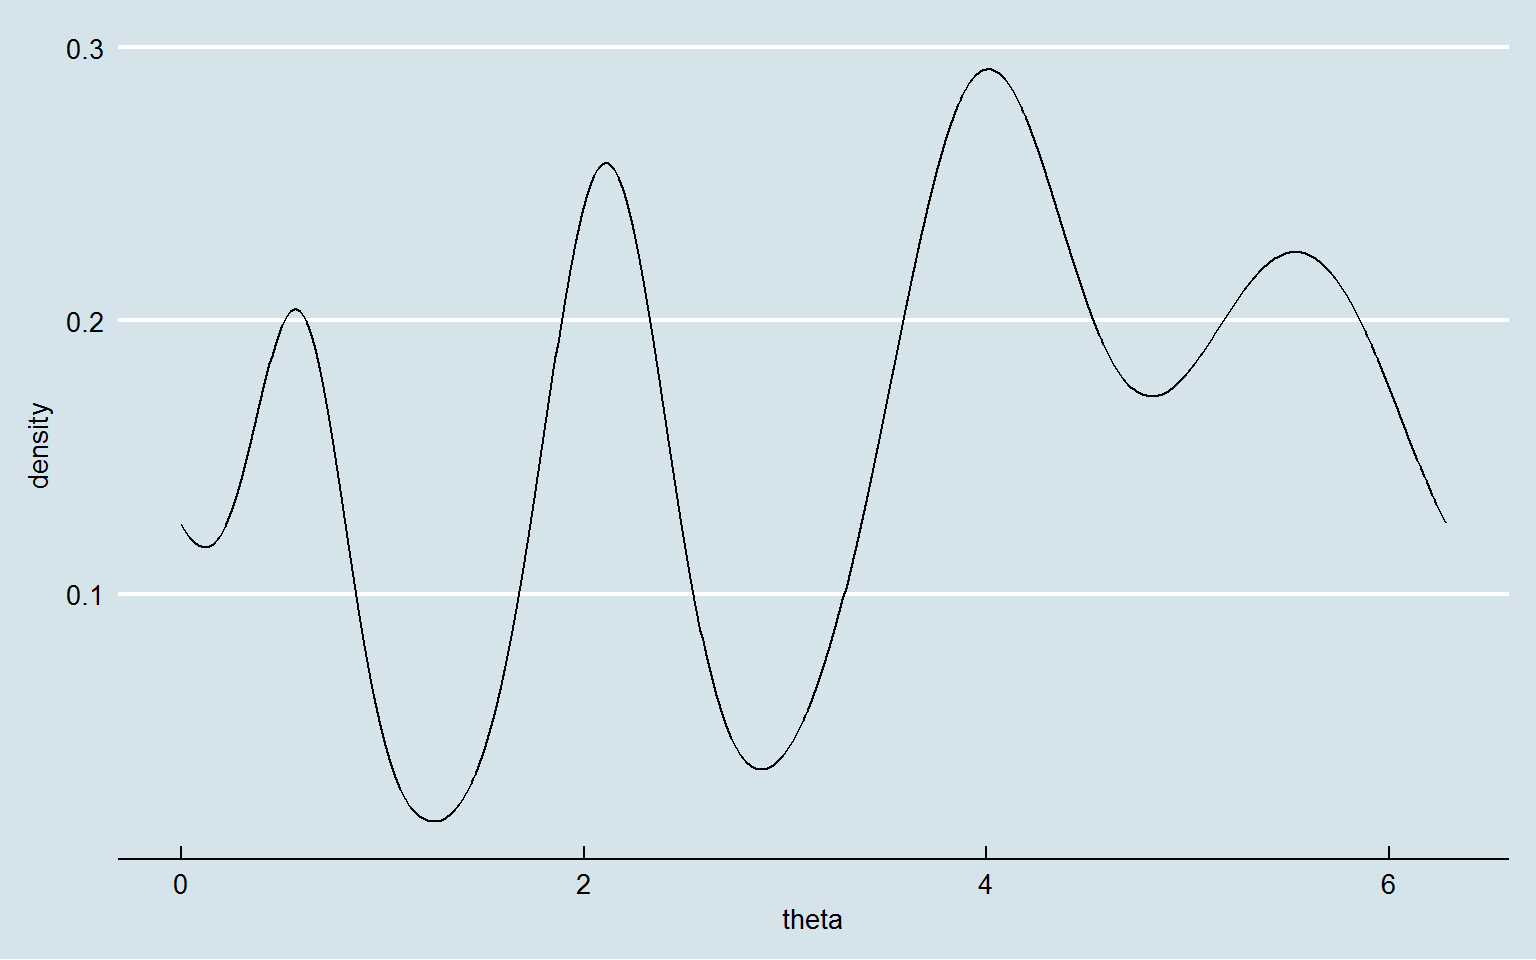
\includegraphics[clip,height= 35mm]{data/mix_von.png}
  \end{center}
 % \caption{Mixture von Mises分布により推定した混合分布}
  \label{vonmix}
 \end{minipage}
  \end{tabular}
\caption{Mixture Projected Normal 分布により推定した混合分布(左), Mixture von Mises分布により推定した混合分布(右)}
\end{figure}


得られた混合分布から, 混合データの分類を行う. 混合分布を構成する, 分布の中で出現確率が最も高いものをそのデータの予測クラスタとする.
横軸を真のクラスタ, 縦軸を予測クラスタとして集計表を示す. 

\begin{table}[H]
\caption{PN 分布によるクラスター推定(左), VM 分布によるクラスター推定(右)}
\begin{tabular}{c}
% 1
\hspace{1.5cm}
\begin{minipage}{0.5\hsize}
\begin{center}
%\caption{PN 分布によるクラスター推定}
\begin{tabular}{|c|c|c|c|c|}
\hline
 &  & \multicolumn{3}{|c|}{Predict} \\ \hline
 &  & 1 & 2 & 3 \\ \hline 
 &1 & 38 & 10 & 352 \\ \cline{2-5}
True
 & 2 & 1 & 192 & 7 \\ \cline{2-5}
 & 3 & 0 & 2  & 298 \\ \cline{2-5}
 & 4 & 93 & 0 & 7 \\ 
\hline
 \end{tabular}
 \end{center}
\end{minipage}

% 2
\hspace{-2.5cm}
\begin{minipage}{0.5\hsize}
\begin{center}
%\caption{VM 分布によるクラスター推定}
\begin{tabular}{|c|c|c|c|c|c|}
\hline
 &  & \multicolumn{4}{|c|}{Predict} \\ \hline
 &  & 1 & 2 & 3 & 4 \\ \hline 
 & 1 & 333 & 10 & 39 & 18 \\ \cline{2-6}
True
 & 2 & 7 & 192 & 1 & 0 \\ \cline{2-6}
 & 3 & 298 & 2  & 0 & 0 \\ \cline{2-6}
 & 4 & 0 & 1 & 94 & 5 \\ 
\hline
\end{tabular}
\end{center}
\end{minipage}

\end{tabular}
\end{table}

%%%%%%%%%%%%%%%%%%%%%%%%%%%%%%%%%%%%%%%%%%%%%%%%%%%%%%%%%%%%%%%%%%%%%%
%%%%%%%%%%%%%%%%%%%%%%%  section5 まとめ %%%%%%%%%%%%%%%%%%%%%%%%%%%%%

\section{まとめ}

現在超球面上のクラスタリングは, テキストマイニングなどの分野に用いられている. 本研究で作成した混合 Projected Normal 分布をテキストマイニングに適用する.

%\newpage
\addcontentsline{toc}{section}{参考文献} %目次に参考文献を入れる

%必要になる
%\newpage
%\section{付録}

%参考文献を引用する際に必要なコマンド
\bibliographystyle{jplain}
\bibliography{bunken}

%%%%%%%%%%%%%%%%%%%%%%%%%%%%%%%%%%%%%%%%%%%%%%%%%%%%%%%%%%%%%%%%%%%
%%%%%%%%% 参考文献用 bibtexから呼び出すページ %%%%%%%%%%%%%%%%%%%%%%%%%%

\newpage

関係ないページです!

Presnell(1998) \cite{PML}

Wang and Gelfand (2013) \cite{PN1}

D. Hemandez(2017) \cite{GPN}

Dhillon and Modha(2001) \cite{SKMcluster}

Gopal and Yang(2014) \cite{Gopal}

\if0
%%%%%%%% 図の挿入用 %%%%%%%%%%%%%%
\vspace{-0.3cm}
\begin{figure}[H]
\begin{center}
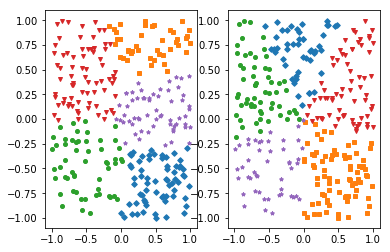
\includegraphics[clip,height= 35mm]{data/kmeans+skmeans.png}
\end{center}
 \vspace{-0.9cm}
\caption{k-meansによるクラスタリング(左), skmeansによるクラスタリング(右)}
\label{skmeans}
\end{figure}

%%%%%%%% 回り込み図の挿入用 %%%%%%%%%%%%%%
\begin{wrapfigure}[10]{r}[5mm]{70mm}
\vspace{-0.6cm}
\centering
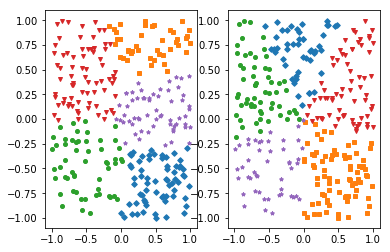
\includegraphics[keepaspectratio,width=70mm]{data/kmeans+skmeans.png}
\vspace{-1cm}
\caption{k-meansによるクラスタリング(左), skmeansによるクラスタリング(右)}
\label{kmeans}
\end{wrapfigure}
\fi

\end{document}

%\begin{table}[H]
%\begin{center}
%\caption{条件付確率表(CPT)}   %キャプション
%\label{cpt}   %ラベル
%\begin{tabular}{|c||c|c|c|}   %{}で文字の揃え方を指定
%\hline
% & $Pa(X_{j})=x_{1}$ & \dots & $Pa(X_{j})=x_{m}$
%\\ \hline
%$X_j=y_1$ & $p(y_1|Pa(X_j)=x_1)$ & \dots & $p(y_1|Pa(X_j)=x_m)$
%\\ \hline
%$\vdots$ & $\vdots$ & $\ddots$ & $\vdots$
%\\ \hline
%$X_j=y_n$ & $ p(y_n|Pa(X_j)=x_1)$ & \dots & $p(y_n|Pa(X_j)=x_m)$
%\\ \hline
%\end{tabular}
%\end{center}
%\end{table}
